\section{Introduction}
% \subsection{Motivation}
Over the decades since its inception, the field of computer science has become increasingly complex and confusing.
This has caused students today to lose track of the picture at large and instead specialize on specific aspects of the field.
Shimon Schocken and Noam Nisam believe that this is an issue and that the best way to understand how computers actually work is to build one from scratch yourself.~\cite[Preface]{nisan2005}

In order to enable students to take this seemingly impossible approach, Schocken and Nisan developed the Nand to Tetris course in 2004, which gives students the opportunity to build an entire computer system themselves.~\cite{1408798}
The system the participants create over the course of twelve projects is powerful enough to allow for the implementation of complex applications and games.\ref{fig:hackenstein-offiziell}

\begin{center}
  \begin{figure}[ht]
    \centering
    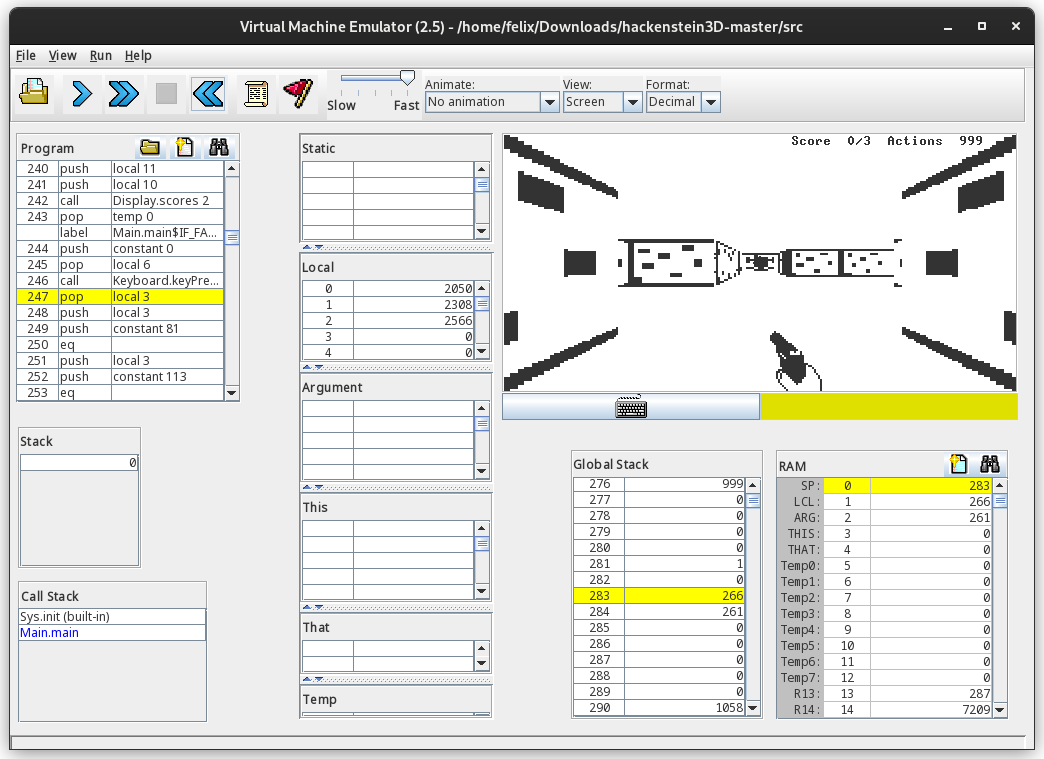
\includegraphics[width=10cm]{fig/hackenstein-offiziell.png}
    \caption{A simple Wolfenstein 3D Clone running in the VM Emulator.}%
    \label{fig:hackenstein-offiziell}
  \end{figure}
\end{center}

To enable students to work on the included projects in a different order than intended, the authors included a hardware simulator to start with and two different emulators, which are capable of emulating the progress of the preceding projects.
Those emulators however are also a frequent point of criticism among course participants, as they increasingly no longer meet the demands of modern users.
Written in Java using the Swing Framework they are not only slow, but also do not adapt to today's higher display resolutions, making it difficult to actually see the contents of the running application~\ref{fig:hackenstein-offiziell}.
It is therefore meaningful to rewrite those emulators in order to make the course more approachable and by extension increase the number of participants.

% \subsection{Contributions}
As part of this work, the two emulators were rewritten as a browser application using WebAssembly. This not only enables support for larger screens and significantly improved performance, but also allows the tools to be used without being installed on the the student's computer.
The new emulator implementations can now be accessed by simply visiting an url in a web browser, and submitting the bytecode or assembly files with a filepicker dialog. The performance has improved significantly, as shown in ~\cref{sec:benchmarks}, enabling users to build even more complex games and applications then before.
Furthermore, both emulators can be compiled to stand-alone executables, that can run the course's test scripts without any user input, allowing teachers and correctors of the course to use the new emulators to assess students submissions.
